\indent En esta secci\'on, mostraremos buenos y malos casos para nuestro algoritmo, y a su vez, daremos el tiempo estimado 
seg\'un la complejidad del algoritmo calculada anteriormente.

Como la complejidad presenta dos variables marcadas, como son las capacidades de las mochilas y la cantidad de objetos, decidimos, para obtener datos m\'as concisos, realizar los testeos dejando constante la cantidad de objetos y/o las capacidades.\\

Luego de realizar varios experimentos, llegamos a la conclusi\'on que, dejando constante la cantidad de objetos y trabajando con las capacidades, el mejor caso para nuestro algoritmo es en el cual \textbf{todas las mochilas presentan las mismas capacidades} ya que de esta forma nuestro algoritmo realiza la misma ejecuci\'on para cada una de las mochilas sin repetidos.\\
A continuaci\'on mostraremos un gr\'afico que representa lo enunciado:

\vspace*{0.3cm} \vspace*{0.3cm}
  \begin{center}
% 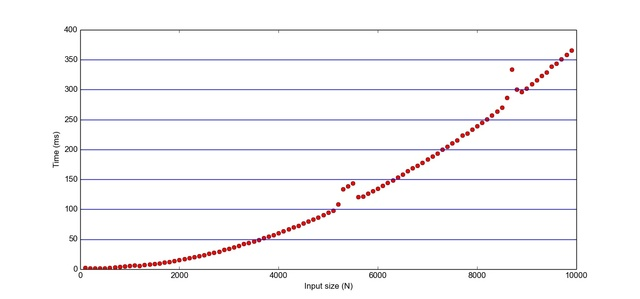
\includegraphics[scale=0.8]{./EJ3/resized2.jpg}
  \end{center}
  \vspace*{0.3cm}

Dividiendo por la complejidad calculada se obtuvo lo siguiente:\\

\vspace*{0.3cm} \vspace*{0.3cm}
  \begin{center}
% 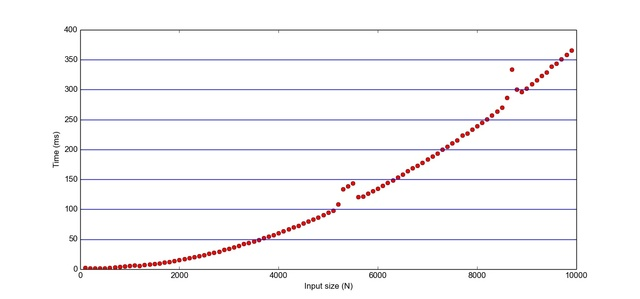
\includegraphics[scale=0.8]{./EJ3/resized2.jpg}
  \end{center}
  \vspace*{0.3cm}
  
Se puede ver en el gr\'afico 3.2 como la funci\'on resultante tiende a 0 cuando las capacidades aumentan.\\

Manteniendo el mismo razonamiento, el peor caso para nuestro algoritmo se da cuando hay \textbf{mochilas con capacidades distintas} ya que el algoritmo deber\'a decidir en que mochila colocar el objeto para que el resultado sea \'optimo. Por consiguiente, mostraremos un gr\'afico que representa lo hablado:\\

\vspace*{0.3cm} \vspace*{0.3cm}
  \begin{center}
% 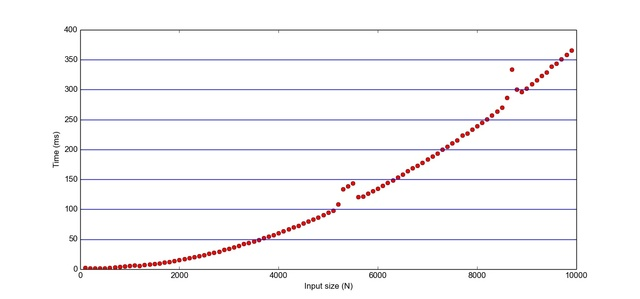
\includegraphics[scale=0.8]{./EJ3/resized2.jpg}
  \end{center}
  \vspace*{0.3cm}

Dividiendo por la complejidad calculada se obtuvo lo siguiente:\\

\vspace*{0.3cm} \vspace*{0.3cm}
  \begin{center}
% 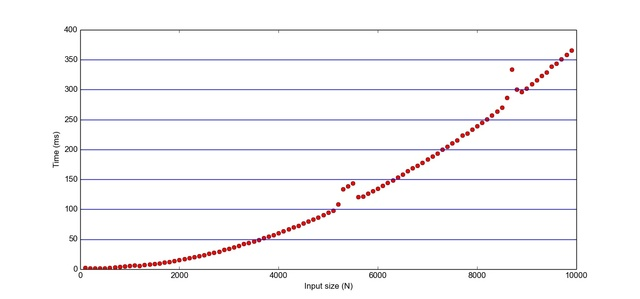
\includegraphics[scale=0.8]{./EJ3/resized2.jpg}
  \end{center}
  \vspace*{0.3cm}
  

Se puede ver, tanto en el gr\'afico 3.2 como 3.4 la funciones resultantes siempre se mantienen por debajo de 1, con lo cual se ve que tanto en el mejor como en el peor caso nuestro algoritmo sigue estando acotado por la complejidad calculada.\\

Luego, como nuestro algoritmo calcula lo mismo para cualquier tipo de objeto, ya sean todos iguales o no, todos ser\'an casos promedios, salvo el caso en el cual no haya ning\'un tipo de objeto que entre en alguna mochila, este caso podr\'iamos tomarlo como \'el mejor ya que nuestro algoritmo corta al ver que no puede colocar ning\'un objeto dentro de alguna mochila.\\
Dejando de lado este caso, el resto de los mismos tendr\'an un tiempo de ejecuci\'on similar.\\

Mostraremos en el siguiente gr\'afico de ejemplo lo hablado recientemente:\\

\vspace*{0.3cm} \vspace*{0.3cm}
  \begin{center}
% 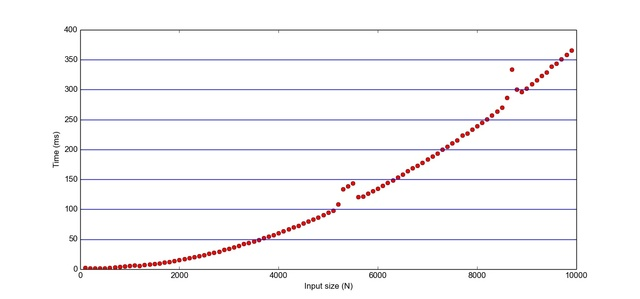
\includegraphics[scale=0.8]{./EJ3/resized2.jpg}
  \end{center}
  \vspace*{0.3cm}